\documentclass[12pt,a4paper]{article}

\usepackage[letterpaper]{geometry}

\usepackage{times}
\geometry{top=1.0in, bottom=1.5in, left=1.0in, right=1.0in}

\usepackage{fancyhdr}
\pagestyle{fancy}
\lhead{}
\rhead{}
\lfoot{}
\rfoot{}

\renewcommand{\headrulewidth}{0pt} 
\renewcommand{\footrulewidth}{0pt} 

\setlength\headsep{0.333in}

\usepackage{fontspec}
%\setmainfont{Times New Roman}

\usepackage{graphicx}

\usepackage{hyperref}

\usepackage{caption}

\usepackage{indentfirst}

\usepackage{setspace}

\usepackage{float}

\usepackage{enumitem}
\usepackage{listings}
\usepackage{color}
\usepackage{xcolor}

\begin{document}

\begin{titlepage}

\newcommand{\HRule}{\rule{\linewidth}{0.5mm}}

\center

\textsc{\LARGE UM - SJTU Joint Institute}\\[1cm]
\textsc{\Large Physics Laboratory I}\\[0.5cm]
\textsc{\large VP141}\\[0.5cm]

\HRule \\[0.4cm]
{
    \bfseries
    {\huge Exercise II}\\[0.3cm]
    {\large Measurement of Fluid Viscosity}\\[0.2cm]
    \HRule \\[1.5cm]
}

\begin{minipage}{0.6\textwidth}

\large
\emph{Name:}\\
Tianyi \textsc{Ge} \\

\emph{Student Number:}\\
516370910168 \\

\emph{Group:}\\
17\\

\emph{Instructor:}\\
Prof. Mateusz \textsc{Krzyzosiak}

\end{minipage}\\[3.5cm]

{\large \today}\\[2cm]

\vfill

\end{titlepage}

%\setmainfont{Times New Roman}
\doublespacing 
\newpage

\section{Theoretical Background}

Moment of inertia of a rigid body about an axis is a quantitative
characteristics that defines the body’s resistance (inertia) to a change of
angular velocity in rotation about that axis. 
This characteristics of the rigid body rotating about a fixed axis is determined
not only by the mass of the body, but also by its distribution. 
The moment of inertia of a rigid body about a certain rotation axis can be
calculated analytically. 
However, if the body has irregular shape or non-uniformly distributed mass, the
calculation may be di cult.
Experimental methods turn out to be more useful in such cases.

\subsection{Laws of Physics Used}

There are mainly two laws of Physics been used in the experiment. Second law of
dynamics for rotational motion can find the relationship between the rotational
acceleration and the torque at the object.

\subsubsection{Second Law of Dynamics for Rotational Motion}

The rotational motion about a fixed axis relates with the component of the
torque about the axis of rotation with the moment of inertia about this axis.
$$ \tau_z = I\beta_z$$
Therefore, the moment of inertia I can be found once the torque and the
resulting angular acceleration are measured.

The moment of inertia is an additive quantity, the moment of inertia of the
combined rigid body AB composed of A and B, about the same axis of rotation, is 
$$ I_{ab} = I_A + I_B $$


\subsubsection{Parallel Axis Theorem}
If the moment of inertia of a rigid body with mass m about an axis through the
body’s center of mass is I0, then for any axis parallel to that axis, the moment
of inertia is
$$ I = I_0 + md^2 $$
where $d$ is the distance between the axes.

\section{Apparatus}
The measurement setup consists of a turntable with an integrated photo-gate
system used for time measurements.
\singlespacing
\begin{itemize}
\item sample
\item turntable
\item photo gate holder
\item pulley
\item string
\item weight
\item photo gate
\item shielding pin
\item cone pulley
\item levelling bolt
\item arm holder
\end{itemize}
\doublespacing

\begin{figure}[H]
\centering
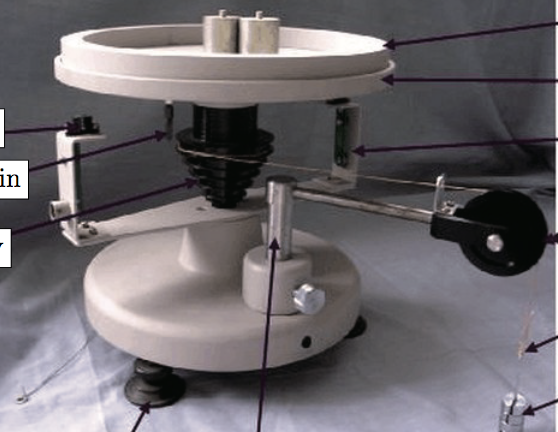
\includegraphics[width=15cm]{fig/app/turntable}
\end{figure}

Since the bearings of the turntable are not frictionless, there will be a
non-zero frictional torque $M_μ$ causing the turntable to decelerate with
angular acceleration $\beta_1$, so that the second law of dynamics for
rotational motion of the empty turntable reads $$   M_\mu = -I_1\beta_1  $$
\section{Procedure}
\begin{enumerate}
\item Measure the mass of the weight, the hoop, the disk, and the cylinder, as
  well as the radius of the cone pulley and the cylinder (follow the
  instructor’s requirements). Calculate the moment of inertia of the hoop and
  the disk analytically.
\item Turn the electronic timer on and switch it to mode 1-2 (single gate,
  multiple pulses). 
\item Place the instrument close to the edge of the desk and stretch the disk
  pulley arm outside, so that the weight can move downwards unobstructed. 
\item Level the turntable with the bubble level.
\item Make the turntable rotating and press the start button on the timer. After
  at least 8 signals are recorded, stop the turntable and record the data in
  your data sheet. 
\item Attach the weight to one end of the string. Place the string on the disk
  pulley, thread through the hole in the arm, and wind the string around the 3rd
  ring of the cone pulley. Adjust the arm holder so that the string goes through
  the center of the hole. 
\item Release the weight and start the timer. Stop the turntable when the weight
  hits the floor. Write down the recorded data. 
\item The angular acceleration can be found by plotting $\theta =k\pi$ against
  $t$ and performing a quadratic fit using data processing software. (The
  magnitude of the angular acceleration is equal to the coefficient next to
  $t^2$ multiplied by two. The uncertainty of the angular acceleration can be
  read directly from the fitting result.) 

  The moment of inertia of the empty turntable is found by using the formulae in
  Section 3 and the data from step 5 and 7. Repeat steps 5--7 with a rigid
  object placed on the turntable. An equaition is used to find the moment of
  inertia of the rigid object. 
\end{enumerate}
The timer’s resolution is $0.0001 s$, and the error is $0.004\%$. 

\section{Calculations and Results}
From the following equaitions,

$$ \tau_z = I\beta_z $$
$$ I_{ab} = I_A + I_B $$
$$ M_\mu = -I_1\beta_1 $$
$$ T = m(g-a)$$

We can derive
$$ m(g-R\beta_2)R-M_\mu=I_1\beta_2 $$
Then we find
$$ I_1=\frac{mR(g-R\beta_2)}{\beta_2-\beta_1} $$
Similarly, if a rigid body with an unknown moment of inertia is placed on the
turntable, we may find 
$$ I_2=\frac{mR(g-R\beta_4)}{\beta_4-\beta_3} $$
Using the fact that the moment of inertia is an additive quantity, the moment of
inertia of the rigid object placed on the turntable, with respect to the axis of
rotation, may be found as the difference 
$$ I_3 = I_2 - I_1 $$

\subsection{Measurement of Angular Acceleration}
Angular acceleration can be derive by investigating the measurement data (k,t),
the corresponding angular position is
$$ \theta = k\pi = \omega_0 t + \frac{1}{2}\beta t^2 $$

\section{Measurement Uncertianty Analysis}

\section{Conclusions and Discussion}

% data sheet

\end{document}